\section{Время-цифровой преобразователь}\label{sec:secTDC}

На~\figref{fig:TDCscheme} приведена условная схема функционирования одного канала ВЦП, дающая представление о причинах сдвига калибровочной таблицы и объясняющая минус в формуле расчёта полного времени.

\begin{figure}[H]
\centering
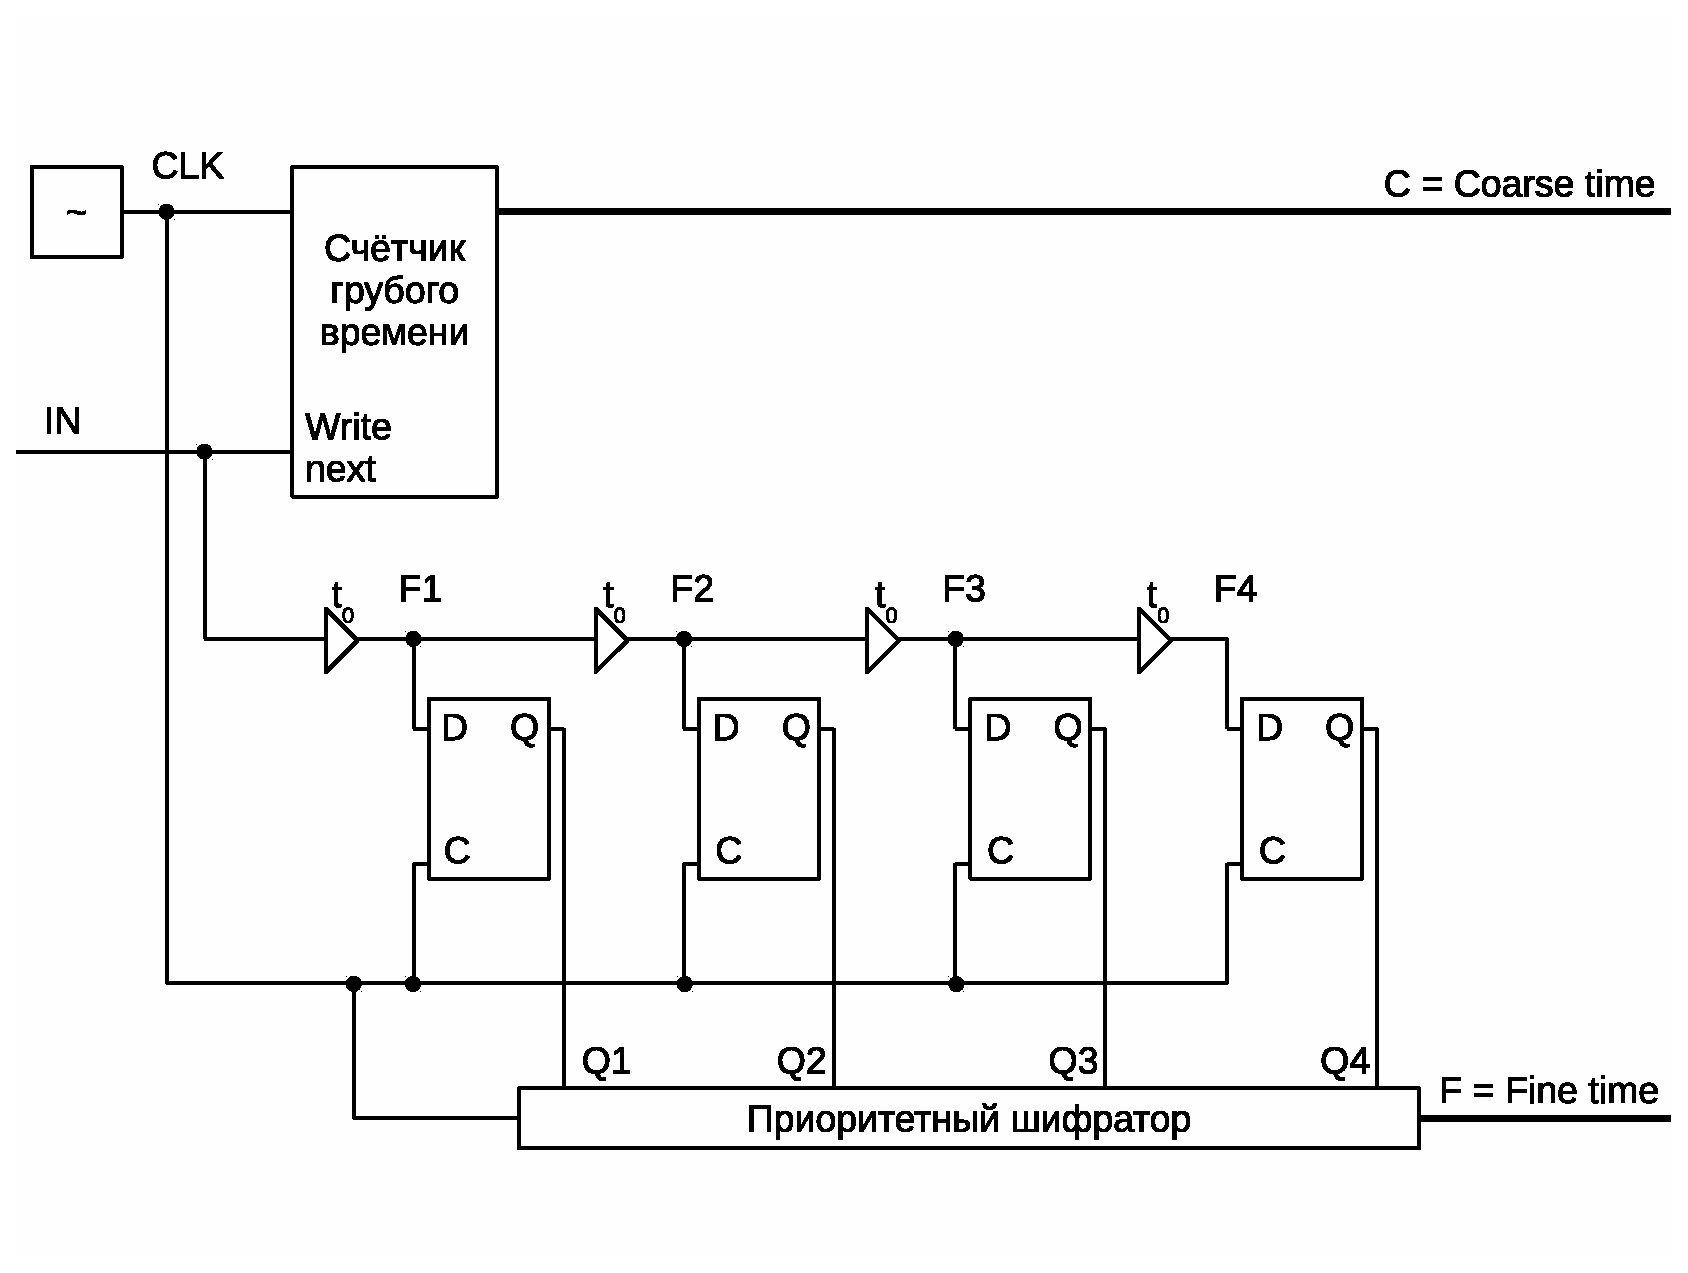
\includegraphics[width=0.7\textwidth]{pictures/TDC.eps}
\caption{Структурная схема одного канала ВЦП.}
\label{fig:TDCscheme}
\end{figure}

Имеется тактовый генератор частотой 200~МГц. Период такого генератора --- 5~нс. Он управляет счётчиком грубого времени. Каждые 5~нс значение грубого времени увеличивается, но не выдаётся на выход. Счётчик точного времени выполнен по технологии Tapped delay line (TDL) --- цифровая линия задержки (DDL) с промежуточными выходами. Используются элементы задержки $t_{0}$, имеющие одинаковые характеристики в пределах некоторой точности. Количество элементов должно быть таким, чтобы полностью заполнить период между двумя отсчётами грубого времени. Регистрируемый фронт, поступающий на вход IN, проходит линию задержки, состоящую из нескольких элементов задержки. По мере прохождения линии фронтом триггеры переключаются из~0~в~1, каждый следующий --- через промежуток времени, равный $t_{0}$. При поступлении следующего фронта от тактового генератора происходит считывание грубого времени и перенос значений выходов триггеров в приоритетный шифратор.

\begin{figure}[H]
\centering
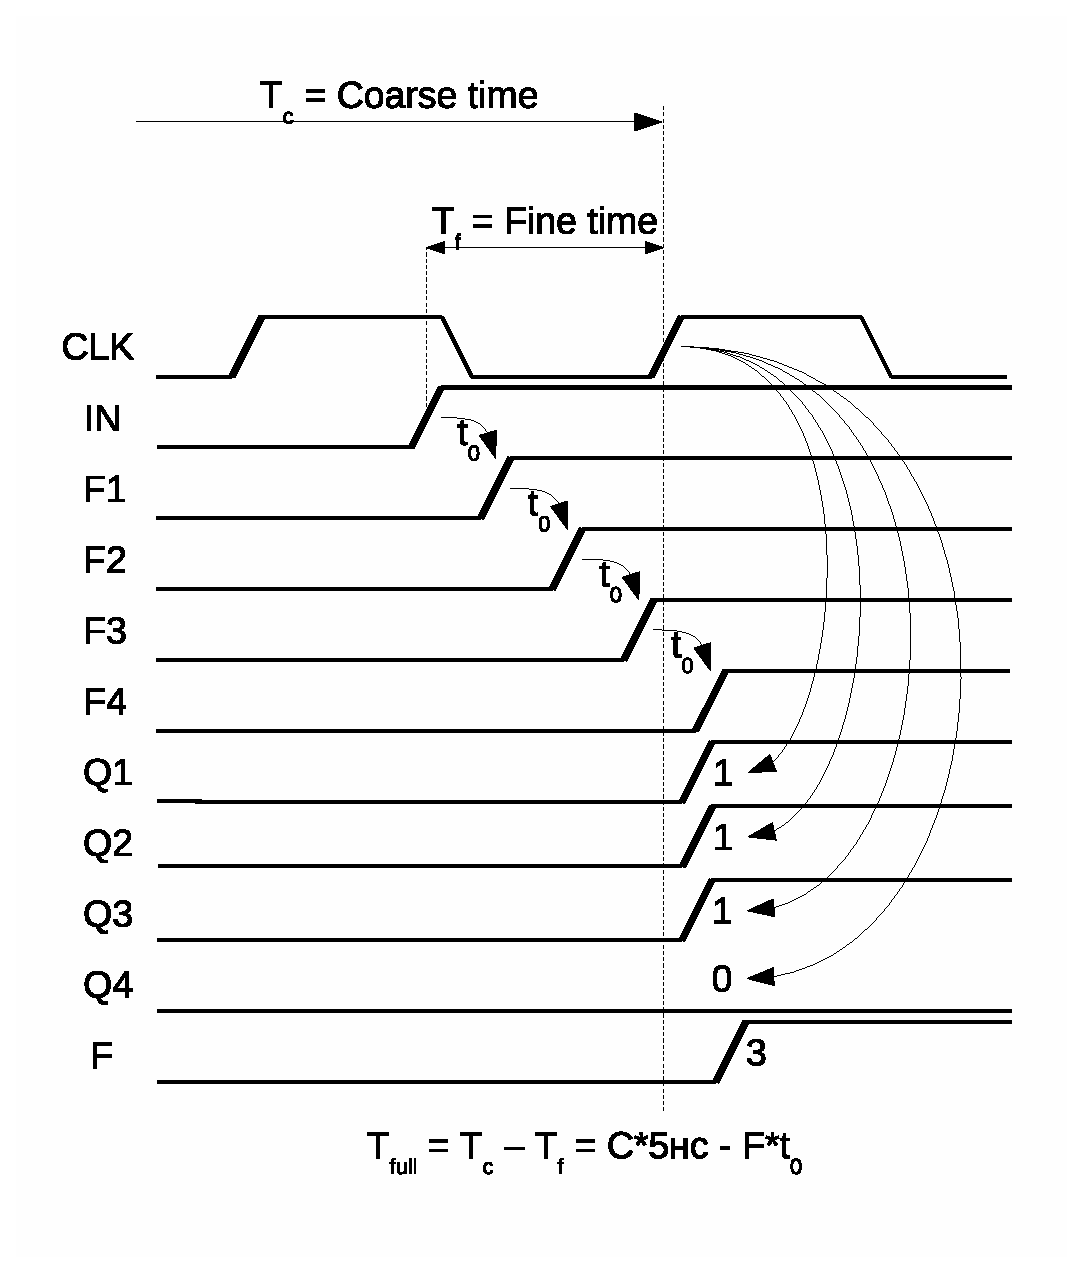
\includegraphics[width=0.7\textwidth]{pictures/TDC_diag.eps}
\caption{Пример временных диаграмм при регистрации входного фронта.}
\label{fig:TDCtimeDiag}
\end{figure}

Отличительная особенность такого шифратора --- индиффирентность к значению на входах $j<i$ при наличии логической единицы на входе $i$. Иными словами, имеет значение только старший бит, а младшие игнорируются. (У обычного шифратора только один вход должен иметь единицу на входе). Шифратор преобразует номер последнего переключившегося триггера в число, обозначающее значение точного времени. Таким образом, точное время должно вычитаться из грубого времени потому что линия задержки измерила время между моментом прихода входного сигнала (start) и моментом прихода следующего отсчёта грубого времени (stop).

Приведена наиболее понятная схема, фактическая же реализация отличается. Например, в качестве элемента задержки может выступать сам триггер. Тогда выход i-го триггера напрямую соединяется со входом (i+1)-го триггера. Используемые нами ВЦП в ППВМ имеют в качестве элемента задержки ячейку матрицы, запрограммированную как полный сумматор.
% [докум. TRB, раздел 10.1.1].

% \todo Очевидно, причесать.

ВЦП разрабатывался так, чтобы интервал 5~нс между двумя отсчётами грубого счётчика разбивался на 512~элементов. Тогда было бы достаточно 9-битного шифратора для формирования значения точного времени. Из-за того что существует также и задержка сигналов в проводниках ненулевой длины, реально таблица может быть сдвинута. Например, значение точного времени~0 должно означать, что входной фронт пришёл одновременно с фронтом от тактового генератора (точнее совсем чуть-чуть раньше). Если учитывать задержку в проводниках на приведённой условной схеме, то получится, что команда считывания шифратору идёт дольше, чем до первого триггера. В таком случае никогда не будет принято нулевого значения и 9~бит для хранения точного времени будет недостаточно. По данной причине сообщение, несущее точное время, имеет длину 10~бит, а все калибровочные таблицы имеют правую границу на значении~1024.

Пример таблицы калибровки точного времени представлен в виде графика на~\figref{fig:CalibTable}. По оси абсцисс откладывается значение счётчика точного времени, а по оси ординат --- значение точного времени в наносекундах.

% \todo Эта картинка дублирует картинку ниже по тексту

\begin{figure}[H]
\centering
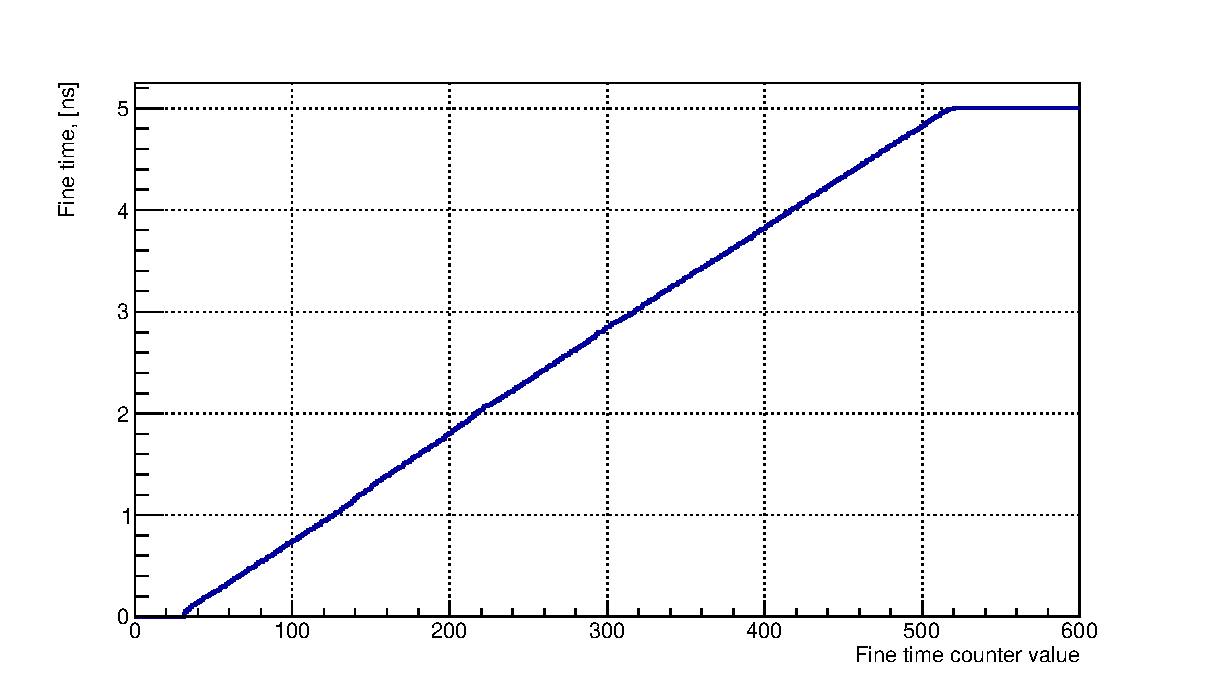
\includegraphics[width=0.7\textwidth]{pictures/CalTable_0010_01.eps}
\caption{Пример таблицы калибровки точного времени.}
\label{fig:CalibTable}
\end{figure}
